\documentclass{beamer}
\usetheme{FINKI}
\usepackage{thumbpdf}
\usepackage{wasysym}
\usepackage{ucs}
\usepackage[T2A]{fontenc}
\usepackage[utf8]{inputenc}
\usepackage{verbatim}
\usepackage{tikz}
\usetikzlibrary{shapes,arrows}
\usepackage{listings}
\renewcommand\mathfamilydefault{\rmdefault}
%\renewcommand*\ttdefault{lcmtt}

\pdfinfo
{
  /Title       (KRS)
  /Creator     (TeX)
  /Author      (Tomche Delev)
}


\title[АВ1]{Аудиториски вежби 1}
\subtitle{Вовед во C\\Околини за развој (IDE)}
\author{Концепти за развој на софтвер}
\date{}
\pgfdeclareimage[width=0.6\paperwidth]{finki_logo}{finki_name}
\titlegraphic{\pgfuseimage{finki_logo}}

\lstset{language=C,captionpos=b,
tabsize=4,frame=lines,
basicstyle=\tiny\ttfamily,
keywordstyle=\color{blue},
commentstyle=\color{lightgray},
stringstyle=\color{violet},
breaklines=true,showstringspaces=false}


\begin{document}

\frame[plain]{\titlepage}
\AtBeginSection[]
{
  \frame
  {
    \frametitle{Содржина}
    \tableofcontents[currentsection,hideallsubsections]
  }
}

\AtBeginSubsection[]
{
  \frame
  {
    \frametitle{Содржина}
    \tableofcontents[sectionstyle=show/hide,subsectionstyle=show/shaded/hide]
  }
}

%%%%%%%%%%%%%%%%%%%%%%%%%%%%%%%%%%%%%%%%%
%%%%%%%%%% Content starts here %%%%%%%%%%
%%%%%%%%%%%%%%%%%%%%%%%%%%%%%%%%%%%%%%%%%
\section{Вовед во програмирање}

\begin{frame}{Програмирање (1)}
\begin{itemize}
\item Програмите што се извршуваат на компјутерот се последователност од \textbf{нули и
единици} и тоа е единствениот јазик што компјутерот го разбира
\item Програмерите пишуваат програми  со помош на јазици кои се разбирливи за
нив, односно \textbf{јазици за програмирање} 
\item Програма напишана во јазик за програмирање ја нарекуваме \textbf{изворна програма}
\end{itemize}
\end{frame}

\begin{frame}{Програмирање (2)}
\begin{itemize}
  \item За пишување програми често се користат \textbf{околини за развој}
  \item Програмата се внесува преку текстуален уредувач
  \item Потоа се врши преведување на програмата (\textbf{компајлирање})
  \item Со тоа се создава \textbf{извршна програма} т.е. програма
напишана во јазикот на компјутерот
\end{itemize}
\end{frame}

% Define block styles
\tikzstyle{block} = [rectangle, draw, fill=blue!20,
text width=5em, text centered, rounded corners, minimum height=4em]
\tikzstyle{line} = [draw, -latex']

\begin{frame}[fragile,shrink=20]{Тек на преведување и извршување}

\begin{center}
Фаза 1 - преведување на програмата
\begin{tikzpicture}[node distance = 3cm, auto]
    % Place nodes
    \node [block] (compiler) {Преведувач\\(компајлер)};
    \node [block, below of=compiler, node distance=2cm] (source) {Изворна
    програма}; 
    \node [block, right of=compiler] (computer) {Компјутер};
    \node [block, right of=computer] (executable) {Програма во меморија};
    % Draw edges
    \path [line] (compiler) -> node {} (computer);
    \path [line] (source) -| node {} (computer);
    \path [line] (computer) -> node {} (executable);
\end{tikzpicture}
\end{center}
\begin{center}
Фаза 2 - извршување на програмата
\begin{tikzpicture}[node distance = 3cm, auto]
    % Place nodes
    \node [block] (programm) {Програма во меморија};
    \node [block, below of=programm] (data) {Влезни податоци};
    \node [block, right of=programm] (computer) {Компјутер};
    \node [block, text width=3cm, right of=computer] (executable) {Резултат од
    извршувањето на програмата};
    % Draw edges
    \path [line] (programm) -> node {} (computer);
    \path [line] (data) -| node {} (computer);
    \path [line] (computer) -> node {} (executable);
\end{tikzpicture}
\end{center}
\end{frame}


\begin{frame}{Вовед во програмскиот јазик C}
\begin{itemize}
\item Развиен во лабораториите на Bell во периодот од 1969 од 1973 од страна на Dennis Ritchie
\item Еден од најшироко употребуваните јазици за програмирање со општа намена на сите времиња
\item Има огромно влијание во создавањето на многу други јазици за програмирање
	\begin{itemize}
	\item C++
	\item Objective C
	\item PHP
	\item Java
	\end{itemize}
\end{itemize}
\end{frame}

\begin{frame}[fragile]{Синтакса на C}

  \begin{block}{Азбуката е множество на следните дозволени симболи:}
  \begin{verbatim}
  	a-z, A-Z, 0-9 и ~!@#$%^&*()-+={}[]:;'"<>?/._  
  \end{verbatim}
  \end{block}

	\begin{alertblock}{Внимание!}
	Компајлерот разликува големи и мали букви!
	\end{alertblock}

	Од азбуката на C се формираат зборови кои може да бидат:
	\begin{enumerate}
	\item Клучни зборови
	\item Бројни и симболички константи
	\item Идентификатори
	\item Стрингови (низи од знаци)
	\item Оператори
	\end{enumerate}

\end{frame}

\begin{frame}{Синтакса на C}

  	\begin{block}{Множество на клучни зборови (32)}

  	\begin{tabular}{c c c c}
		\texttt{auto} & \texttt{double} & \texttt{int} & \texttt{struct} \\
		\texttt{break} & \texttt{else} & \texttt{long} & \texttt{switch} \\
		\texttt{case} & \texttt{enum} & \texttt{register} & \texttt{typedef} \\
		\texttt{char} & \texttt{extern} & \texttt{return} & \texttt{union} \\
		\texttt{const} & \texttt{float} & \texttt{short} & \texttt{unsigned} \\
		\texttt{continue} & \texttt{for} & \texttt{signed} & \texttt{void} \\
		\texttt{default} & \texttt{goto} & \texttt{sizeof} & \texttt{volatile} \\
		\texttt{go} & \texttt{if} & \texttt{static} & \texttt{while}
  	\end{tabular}
  	\end{block}
\end{frame}

\begin{frame}[fragile]{Структура на програма во C}

	Севкупниот изворен код кој се пишува во програмскиот јазик C е организиран во функции
	\linebreak
	
	\begin{columns}[t]
		\column{.5\textwidth}
			\begin{block}{Програма во C}
				\begin{lstlisting}
				int main() {
				    deklaracija_na_promenlivi;
				    programski_naredbi;
				}
				\end{lstlisting}
			\end{block}
		\column{.5\textwidth}
			\begin{block}{Програма во Паскал}
				\begin{lstlisting}
				Program ime_na_programata;
				var deklaracija_na_promenlivi;
				begin
				    programski_naredbi;
				end.
				\end{lstlisting}
			\end{block}
	\end{columns}

\end{frame}

\begin{frame}[shrink=10]{Функции во C}
 	\hfill
  	\begin{block}{\texttt{main}}
  		Главна фунција во C
  	\end{block}
  	
  	\begin{block}{\texttt{()}}
		Во мали загради се примаат влезните аргументи
  	\end{block}
  	
  	\begin{block}{\texttt{int}}
		Видот на податокот кој се враќа како резултат стои пред името на функцијата
  	\end{block}
  	
  	\begin{block}{\texttt{\{\}}}
		Телото на функцијата започнува со \{, а завршува со \}
  	\end{block}

	\begin{block}{\texttt{;}}
  	Сите наредби се одделуваат меѓусебно со \texttt{;}
  	\end{block}

\end{frame}

\begin{frame}[fragile]{Употреба на коментари}
	\begin{itemize}
		\item За дополнително до објаснување или документирање на изворниот код се користат коментари
		\item Во C постојат два видови на коментари
		\begin{enumerate}
			\item коментари во еден ред
			\item коментари во повеќе редови
		\end{enumerate}	
		
	\end{itemize}
		
	\begin{columns}[t]
		\column{.5\textwidth}
			\begin{block}{1. Коментар во еден ред}
				\begin{verbatim}
				\\ komentar vo eden red
				\end{verbatim}
			\end{block}
		\column{.5\textwidth}
			\begin{block}{2. Коментар во повеќе редови}
				\begin{verbatim}
				\* Komentar 
				   vo povekje redovi */
				\end{verbatim}
			\end{block}
	\end{columns}		

\end{frame}

\begin{frame}[fragile]{Примери}
	\begin{exampleblock}{Пример 1}
		\begin{lstlisting}
			#include <stdio.h>
			// glavna funckija
			int main() {
			    /* funkcija za pecatenje na ekran */
			    printf("Dobredojdovte na FINKI!\n");
			    return 0;
			}
		\end{lstlisting}
	\end{exampleblock}
\end{frame}

\begin{frame}{Структура на програма во C (проширена)}
	\begin{columns}
		\column{.2\textwidth}
		\textbf{INCLUDE} секција
		\column{.8\textwidth} содржи \texttt{\#include} изрази за вклучување на надворешни библиотеки, односно користење веќе дефинирани надворешни функции
	\end{columns}
	\hfill
	\linebreak
	\begin{columns}
		\column{.2\textwidth}
		\textbf{DEFINE} секција
		\column{.8\textwidth} содржи \texttt{\#define} изрази за декларирање на константи и податочни типови
	\end{columns}	
	\hfill
	\linebreak
	\begin{columns}
		\column{.2\textwidth}
		...
		\column{.8\textwidth} дефинирање на глобални променливи и функции
	\end{columns}
	\hfill
	\linebreak
	\begin{columns}
		\column{.2\textwidth}
		\texttt{int main()}
		\column{.8\textwidth} главна функција
	\end{columns}
\end{frame}

\begin{frame}{Претпроцесор}
\begin{itemize}
	\item Во C преведувањето (компајлирањето) на програмите го извршуваат:
	\begin{itemize}
		\item претпроцесорот
		\item компајлерот
	\end{itemize}
	\item Претпроцесорот се управува со помош на т.н. директиви
	\begin{itemize}
		\item Секоја директива започнува со \texttt{\#}
	\end{itemize}
\end{itemize}
\end{frame}

\begin{frame}{Датотека со заглавја}
\begin{itemize}
	\item Една примена на претпроцесорски наредби е вклучување на „датотека со заглавија“ (анг. header file)
	\begin{itemize}
		\item Се користи за декларација на функции и променливи на одредена предефинирана библиотека
		\item Корисниците ја вклучуваат „датотеката за заглавија“ со цел да ги користат функциите и надворешните променливи
	\end{itemize}
	\item Вклучување се врши со претпроцесорската директива \texttt{\#include}
	\begin{itemize}
		\item Наредбата \texttt{\#include} предизвикува копија од даденa датотека да се вклучи на местото каде што е испишана директивата
	\end{itemize}
\end{itemize}
\end{frame}

\begin{frame}[fragile]{Форми на \texttt{include}}
\begin{itemize}
	\item Има две форми на оваа директива:
	\begin{itemize}
		\item датотеката која се вклучува може да биде ставена во наводници(""), 
		\item или во аголни загради (<>)
	\end{itemize}
	\begin{exampleblock}{Пример}
		\begin{verbatim}
		#include <imedatoteka.h>
		#include "imedatoteka.h"
		\end{verbatim}
	\end{exampleblock}
	\item Разликата е во локацијата во која препроцесорот јa бара датотеката која треба да ја вклучиме
	\begin{itemize}
		\item Со аголни загради (се користат за датотеки од стандардните библиотеки) 
		\item Со наводници (препроцесорот прво ја бара датотеката во истиот директориум каде што се наоѓа С датотеката која треба да се компајлира)
	\end{itemize}
\end{itemize}

\end{frame}

\begin{frame}{Променливи (variables)}
\begin{itemize}
\item Променливите се симболички имиња за места во меморијата во кои се чуваат некакви вредности
\item Сите променливи пред да се користат треба да се \emph{декларираат}
\item Со секое ново сместување на вредност во променливата, старата вредност се брише
\end{itemize}

Начин на декларација на променливи:
\linebreak
\begin{columns}
		\column{.32\textwidth} \fbox{Вид на променливата}
		\column{.32\textwidth} \fbox{Име на променливата}
		\column{.05\textwidth} \fbox{ = }
		\column{.26\textwidth} \fbox{Почетна вредност}
		\column{.05\textwidth} \fbox{ ; }
\end{columns}	

\end{frame}

\begin{frame}{Видови на променливи}
\Large{Видови на променливи во C}
\linebreak
\linebreak
\begin{tabular}{c|c|c}
\textbf{Цели броеви} & \textbf{Знаковни} & \textbf{Децимални}\\
\hline
\texttt{int} & \texttt{char} & \texttt{float} \\
\hline
\texttt{short} & & \texttt{double} \\
\hline
\texttt{long} & &
\end{tabular}
\end{frame}

\begin{frame}{Дефинирање на имиња на променливи}
\begin{itemize}
\item При именувањето на променливите може да се користат:
\begin{itemize}
\item мали букви од a до z;
\item големи букви од A до Z;
\item цифри од 0 до 9 (не смее да започнува со цифра);
\item знак за подвлекување \_ кој се третира како буква (не е препорачливо да започнува со \_);
\end{itemize}
\end{itemize}
\begin{alertblock}{Треба да се внимава!}
\begin{itemize}
\item најчесто должината на имињата на променливите е до 32 знаци
\item С ги разликува малите и големите букви!
\end{itemize}
\end{alertblock}
\end{frame}

\begin{frame}[fragile]{Примери}
	\begin{exampleblock}{Пример 2}
		\begin{lstlisting}
			#include <stdio.h>

			int main() {
			    int a, b, c;
			    a = 5;
			    b = 10;
			    c = a + b;
			    return 0;
			}
		\end{lstlisting}
	\end{exampleblock}
\end{frame}

\begin{frame}{Константи}
\begin{itemize}
\item Со помош на константи се означуваат вредности кои не се менуваат во текот на извршувањето на програмата
\item Секоја константа припаѓа на некој од податочните видови
\item Во C постојат неколку типови на константи:
\begin{itemize}
\item децимални: \texttt{1, -23, 15}
\item октални: \texttt{015, 035, 0205}
\item хексадецимални: \texttt{0x25, 0xA4C}
\item реални: \texttt{3.5F, -2.845F, 1.34e-9}
\item знаковни: \texttt{'a', '\_', 'e'}
\item текстуални: \texttt{" ", "Koncepti za razvoj na softver"}
\end{itemize}
\end{itemize}
\end{frame}

\begin{frame}{Одредување на типот на константите}
\begin{itemize}
\item Одредувањето на типот на променливите е едноставно (се гледа од самата декларација на променливата)
\item Константите не се декларираат и нивниот тип се одредува преку начинот на кој се напишани:
\begin{itemize}
\item Броевите кои содржат "." или "е" се {\color{blue}\texttt{double}}: \texttt{3.5, 1е-7, -1.29е15}
\item За наместо double да се користат {\color{blue}{\texttt{float}}} константи на крајот се додава "F": \texttt{3.5F, 1e-7F}
\item За {\color{blue}\texttt{long double}} константи се додава "L": \texttt{1.29е15L, 1e-7L}
\item Броевите без ".", "е" или "F" се {\color{blue}\texttt{int}}: \texttt{1000, -35}
\item За {\color{blue}\texttt{long int}} константи се додава "L": \texttt{9000000L}
\end{itemize}
\end{itemize}
\end{frame}

\begin{frame}[fragile]{Именувани константи (1)}
\Large{Именуваните константи се креираат со користење на клучниот збор \texttt{const}}
\begin{exampleblock}{Пример 3}
		\begin{lstlisting}
			#include <stdio.h>

			int main() {
			    const long double pi = 3.141592653590L;
			    const int denovi_vo_nedelata = 7;
			    const nedela = 0; /* po default int */
			    denovi_vo_nedelata = 1; /* greshka */
			}
		\end{lstlisting}
	\end{exampleblock}
\end{frame}

\begin{frame}[fragile]{Именувани константи (2)}
Именуваните константи може да се креираат и со користење на претпроцесорот и за нив по правило се користат големи букви
	\begin{exampleblock}{Пример 3}
		\begin{lstlisting}
			#include <stdio.h>
			#define PI 3.141592653590L
			#define DENOVI_VO_NEDELATA 7
			#define NEDELA 7		
			int main() {
			    long double pi = PI;
			    int den = NEDELA;
			}
		\end{lstlisting}
	\end{exampleblock}
\end{frame}

\begin{frame}{Оператори}
\begin{itemize}
\item Операторите се користат за градење на изрази, при што операциите се изведуваат од лево надесно со што се применува правилото на приоритет на операторите во нивното изведување
\item Постојат три видови на оператори
\begin{itemize}
\item Аритметички оператори
\item Релациони оператори
\item Логички оператори
\end{itemize}
\end{itemize}
\end{frame}

\begin{frame}{Аритметички оператори}
Се применуваат на броеви (цели или децимални)
\linebreak
\begin{center}
\begin{tabular}{c|c}
\textbf{Оператор} & \textbf{Операција}\\
\hline
\texttt{+} & Собирање \\
\texttt{-} & Одземање \\
\texttt{*} & Множење \\
\texttt{/} & Делење \\
\texttt{\%} & Делење по модул
\end{tabular}
\end{center}
\end{frame}

\begin{frame}{Релациони оператори}
Се применуваат над било кои споредливи типови на податоци, а резултатот е цел број 0 (неточно) или 1 (точно).
\begin{center}
\begin{tabular}{c|c}
\textbf{Оператор} & \textbf{Значење}\\
\hline
\texttt{<} & Помало \\
\texttt{<=} & Помало еднакво \\
\texttt{>} & поголемо \\
\texttt{>=} & поголемо еднакво \\
\texttt{==} & еднакво \\
\texttt{!=} & различно
\end{tabular}
\end{center}
\end{frame}

\begin{frame}{Логички оператори}
Се користат најчесто во комбинација со релационите оператори за формирање на сложени логички изрази, кои повторно враќаат резултат 0 или 1
\linebreak
\begin{center}
\begin{tabular}{c|c}
\textbf{Оператор} & \textbf{Операција}\\
\hline
\texttt{\&\&} & Логичко И \\
\texttt{||} & Логичко ИЛИ \\
\texttt{!} & Негација
\end{tabular}
\end{center}
\end{frame}

\begin{frame}[fragile]{Дополнителни оператори}
\begin{itemize}
\item Оператор за доделување =
\item Оператори за инкрементирање и декрементирање 
\begin{verbatim}
++, --
\end{verbatim}
\item Користење на операторите + и – на унарен начин
  \begin{verbatim}
	X = + Y;
	X = - Y;
  \end{verbatim}
\item Двојни оператори
\begin{itemize}
\item Комбинација од оператор за доделување и друг оператор 
\begin{verbatim}
(+=, -=, *=, /=, %=)
\end{verbatim}
\end{itemize}
\end{itemize}
\end{frame}

\begin{frame}[fragile]{Оператор за доделување =}
\begin{itemize}
\item Сите изрази имаат вредност, дури и оние кои содржат =
\item Вредноста на таков израз е вредноста на изразот кој се наоѓа на десна страна
\item Затоа е можно и доделување од следниот облик:
\end{itemize}
\begin{verbatim}
    x = (y = 10) * (z = 5);
    x = y = z = 20;
\end{verbatim}
\end{frame}	

\begin{frame}[fragile,shrink=5]{Двојни оператори}
\begin{block}{Оператор +=}
\begin{verbatim}
a += 5; // a = a + 5;
a += b * c; // a = a + b * c;
\end{verbatim}
\end{block}
\begin{block}{Оператор -=}
\begin{verbatim}
a -= 3; // a = a – 3;
\end{verbatim}
\end{block}
\begin{block}{Оператор *=}
\begin{verbatim}
a *= 3; // a = a * 3;
\end{verbatim}
\end{block}
\begin{block}{Оператор /=}
\begin{verbatim}
a /= 3; // a = a / 3;
\end{verbatim}
\end{block}
\begin{block}{Оператор \%=}
\begin{verbatim}
a %= 3; // a = a % 3;
\end{verbatim}
\end{block}
\end{frame}	

\begin{frame}[fragile]{Работа со променливи и оператори}
	\begin{exampleblock}{Пример 4}
		\begin{lstlisting}
			#include <stdio.h>	
			int main() {
			    int a;
			    float p;
			    p = 1.0 / 2.0; /* p = 0.5 */
			    a = 5 / 2;     /* a = 2   */
			    p = 1 / 2 + 1 / 8; /* p = 0; */
			    p = 3.5 / 2.8; /* p = 1.25 */
			    a = p; /* a = 1 */
			    a = a + 1; /* a = 2; */
			    return 0;		
			}
		\end{lstlisting}
	\end{exampleblock}
\end{frame}

\begin{frame}[fragile]{Печатење на стандарден излез}
\begin{itemize}
\item Во C не постои наредба за печатење на екран
\item Се користи готова функција од библиотеката за стандарден влез и излез \texttt{stdio.h} (\textbf{st}andar\textbf{d} \textbf{i}nput/\textbf{o}utput)
\large{\texttt{\#include <stdio.h>}}
\item Функцијата која се употребува е:
\end{itemize}
\begin{verbatim}
int printf(kontrolna_niza, lista_na_argumenti)
\end{verbatim}
\begin{itemize}
\item Контролната низа содржи било каков текст, ознаки за форматот на печатење на аргументите предводени со \% 
или специјални знаци кои започнуваат со \textbackslash. 
\item Ознаките за форматот на печатење се одредуваат според видот на променливата чија вредноста треба да се испише.
\end{itemize}
\end{frame}

\begin{frame}{Ознаки за форматот на печатење}
\begin{scriptsize}
\begin{tabular}{|c|l|}
\hline \textbf{Ознака} & \textbf{Објаснување} \\ 
\hline \texttt{\%d} & за цели броеви \\ 
\hline \texttt{\%i} & за цели броеви \\ 
\hline \texttt{\%c} & за знаци \\ 
\hline \texttt{\%s} & за низа од знаци \\ 
\hline \texttt{\%e} & реален број во технички формат (е) \\ 
\hline \texttt{\%E} & реален број во технички формат (Е) \\ 
\hline \texttt{\%d} & реален број во децимален формат \\ 
\hline \texttt{\%f} & реален број во пократкиот од форматите \%е и \%f \\ 
\hline \texttt{\%g} & реален број во пократкиот од форматите \%Е и \%f \\  
\hline \texttt{\%u} & цел број без предзнак \\ 
\hline \texttt{\%o} & октален цел број без предзнак \\ 
\hline \texttt{\%x} & хексадецимален цел број без предзнак (мали букви) \\ 
\hline \texttt{\%X} & хексадецимален цел број без предзнак (мали букви) \\ 
\hline \texttt{\%p} & прикажува покажувач \\ 
\hline \texttt{\%n} & бројот на испишани знаци се доделува на аргументот \\ 
\hline \texttt{\%\%} & испишување на знакот \% \\ 
\hline 
\end{tabular} 
\end{scriptsize}
\end{frame}

\begin{frame}[fragile]{Примена на функцијата \texttt{printf}}
	\begin{exampleblock}{Пример 5}
		\begin{lstlisting}
		#include <stdio.h>
		int main() {
		   printf(" e zbor dolg %d bukvi.\n", printf("Makedonija"));
		   return 0;
		}
		\end{lstlisting}
	\end{exampleblock}
\end{frame}

\begin{frame}[fragile]{Задача 1}
	Да се напише програма која ќе ја пресметува вредноста на математичкиот израз:
	$ x = \frac{3}{2} + (5 - \frac{46 * 5}{12})$
	\begin{exampleblock}{Решение}
		\begin{lstlisting}
		#include <stdio.h>
		int main() {
		   float x = 3.0 / 2 + (5 - 46 * 5 / 12.0);
		   printf("x = %.2f\n", x);
		   return 0;
		}
		\end{lstlisting}
	\end{exampleblock}
\end{frame}

\begin{frame}[fragile]{Задача 2}
Да се напише програма која за зададена вредност на $ x $ (при декларација на променливата) ќе го пресмета и отпечати на екран $ x^2 $.
	\begin{exampleblock}{Решение}
		\begin{lstlisting}
		#include <stdio.h>
		int main() {
		   int x = 7;
		   printf("Brojot %d na kvadrat e: %d\n", x, x * x);
		   return 0;
		}
		\end{lstlisting}
	\end{exampleblock}
\end{frame}

\begin{frame}[fragile]{Задача 3}
Да се напише програма која за дадени страни на еден триаголник ќе ги отпечати на екран периметарот 
и квадратот од плоштината (нека се работи со \texttt{a=5, b=7.5, c=10.2}).
	\begin{exampleblock}{Решение}
		\begin{lstlisting}
		#include <stdio.h>
		int main() {
		   float a = 5;
		   float b = 7.5;
		   float c = 10.2;
		   float L = a + b + c;
		   float s = L / 2;
		   float P = s * (s - a) * (s - b) * (s - c);
		   printf("Perimetarot e: %.2f\n", L);
		   printf("Plostinata na kvadrat e: %.2f\n", P);
		   return 0;
		}
		\end{lstlisting}
	\end{exampleblock}
\end{frame}

\begin{frame}[fragile]{Задача 4}
Да се напише програма за пресметување на аритметичката средина на броевите 3, 5 и 12.
	\begin{exampleblock}{Решение}
		\begin{lstlisting}
		#include <stdio.h>
		int main() {
		   int a = 3, b = 5, c = 12;
		   float as = a + b + c / 3.0;
		   printf("Aritmetickata sredina e: %.2f\n", as);
		   return 0;
		}
		\end{lstlisting}
	\end{exampleblock}
\end{frame}

\begin{frame}[fragile]{Задача 5}
Да се напише програма која ќе ги отпечати на екран остатоците при делењето на бројот 19 со 2, 3, 5 и 8.
	\begin{exampleblock}{Решение}
		\begin{lstlisting}
		#include <stdio.h>
		int main() {
		   int a = 19;
		   printf("Ostatok pri delenje na %d so 2: %d\n", a, a % 2);
		   printf("Ostatok pri delenje na %d so 3: %d\n", a, a % 3);
		   printf("Ostatok pri delenje na %d so 5: %d\n", a, a % 5);
		   printf("Ostatok pri delenje na %d so 8: %d\n", a, a % 8);
		   return 0;
		}
		\end{lstlisting}
	\end{exampleblock}
\end{frame}

\section{Околини за развој (IDE)}

\begin{frame}{Елементи на околините за развој}
Околината за развој е составена од повеќе програми, кои го олеснуваат
целокупниот развој на една програма
\begin{itemize}
  \item текст уредувач (text editor)
  \item преведувач (компајлер - compiler)
  \item дебагер (debugger)
  \item интеграција на библиотеки со функции
  \item поврзувач (linker)
\end{itemize}
\end{frame}

\begin{frame}{Текст уредувач (text editor)}
\begin{itemize}
  \item Програма која овозможува внесување и уредување на текстот на изворната
  програма
  \item Овозможува зачувување на програми и вчитување на веќе напишани програми
  за нивно повторно уредување 
  \item Означување на клучните зборови и команди во изворната програма (syntax
  highlighting)
\end{itemize}
\end{frame}

\begin{frame}{Текст уредувач (text editor)}
\begin{itemize}
  \item Ја преобразува (преведува) изворната програма од јазикот за програмирање
  во кој е напишана во јазик разбирлив за компјутерот
  \item Се разликуваат два вида преведувачи: \textbf{интерпретери} и \textbf{компајлери} 
  \item Интерпретер е преведувач кој ја \emph{обработува одделно секоја команда}, ја
  проверува за грешки и ја извршува, по што поминува на следната команда  итн.
  \item Компајлер е преведувач кој ја \emph{обработува целата програма}, ја проверува
  за грешки и ја преведува, по што се добива извршната програма.
  \begin{itemize}
  \item Така добиената извршна програма може да се извршува
  \end{itemize}
\end{itemize}
\end{frame}

\begin{frame}{Дебагер (debugger)}
\begin{itemize}
  \item Компајлерите и интерпретерите ги откриваат грешките (синтаксички) во
  програмата поради не правилно користење на јазикот за програмирање
  \item Друг вид на грешки се логичките грешки
  \begin{itemize}
  \item Програмата не го прави тоа за кое што е наменета 
  \item Се откриваат многу тешко
  \end{itemize}
  \item Дебагер е програма која помага при барање на логичките грешки
  \begin{itemize}
  \item Овозможува следење на извршувањето на програмата чекор по чекор
  \end{itemize}
\end{itemize}
\end{frame}

\begin{frame}{Интеграција на библиотеки со функции}
\begin{itemize}
  \item Интегрирање и користење на претходно создадени и проверени модули (потпрограми), уште наречени и функции
  \item Ваквиот начин на организација на програмите има голем број на предности
  \item Повторно искористување на готови функционалности
  \item Пример библиотеки
  \begin{itemize}
    \item За управување со стандардниот влез и излез
    \item За стандардни математички операции 
  \end{itemize}
\end{itemize}
\end{frame}

\begin{frame}{Поврзувач (linker)}
\begin{itemize}
  \item Понекогаш програмата е премногу голема за да се напише во една датотека
  \begin{itemize}
    \item различните делови може да се пишуваат од различни програмери.
    \item некои делови од дадена програма можат да бидат искористени и во друга програма 
    \item Одделно компајлираните делови е неопходно да бидат обединети во една
    цела извршна програма со помош на \textbf{поврзувачот}
    \item Друга улога на поврзувачот е да ги „сврзе“ со програмата потребните
     библиотеки со стандардните функции
  \end{itemize}
\end{itemize}

\end{frame}

\begin{frame}{Околини за развој}{(ntegrated Development Environment - IDE}
\begin{itemize}
  \item Сите овие елементи на околината за развој се обединуваат (интегрираат)
  во т.н. интегрирани околини за развој
  \item Пример за IDE е околината која ќе се користи на овој курс, Code::Blocks
\end{itemize}
\begin{center}

\includegraphics[scale=0.5]{images/cb_logo}
\end{center}
\end{frame}

\section{Code::Blocks - инсталација}
\begin{frame}{Code::Blocks - инсталација}
\begin{itemize}
  \item Како да го најдеме и инсталираме Code::Blocks
  \item Code::Blocks е \textbf{слободен софтвер} и може да се најде
  на\linebreak
  \href{http://www.codeblocks.org/downloads}{http://www.codeblocks.org/downloads}
  \item Во централниот дел на страната има три линка: \textbf{Download the binary release}, Download the source code и Retrieve source code from SVN
  \item За наједноставна инсталација се препорачува да се избере првиот линк -
  \textbf{Download the binary release},
\end{itemize}
\end{frame}

\begin{frame}{Code::Blocks – инсталација (2)}
\begin{itemize}
  \item За почетниците се препорачува да ја симнат верзијата што во нејзе
  вклучува \textbf{MinGW} setup
    \begin{itemize}
  \item моментално тоа е линкот \textbf{codeblocks-10.05mingw-setup.exe} кој е наменет за
  корисниците на сите \textbf{Windows} оперативни системи
  \item Со клик на изворот Sourceforge.net се отвора нова страницата која по
  истекот на 5 секунди сама ќе ви понуди опција да ја зачувате датотеката на од вас избрана локација
  \item По зачувувањето на датотеката следете ги инструкциите за инсталирање
    \end{itemize}
\end{itemize}
\end{frame}

\begin{frame}{Code::Blocks – главен прозорец}
\begin{center}
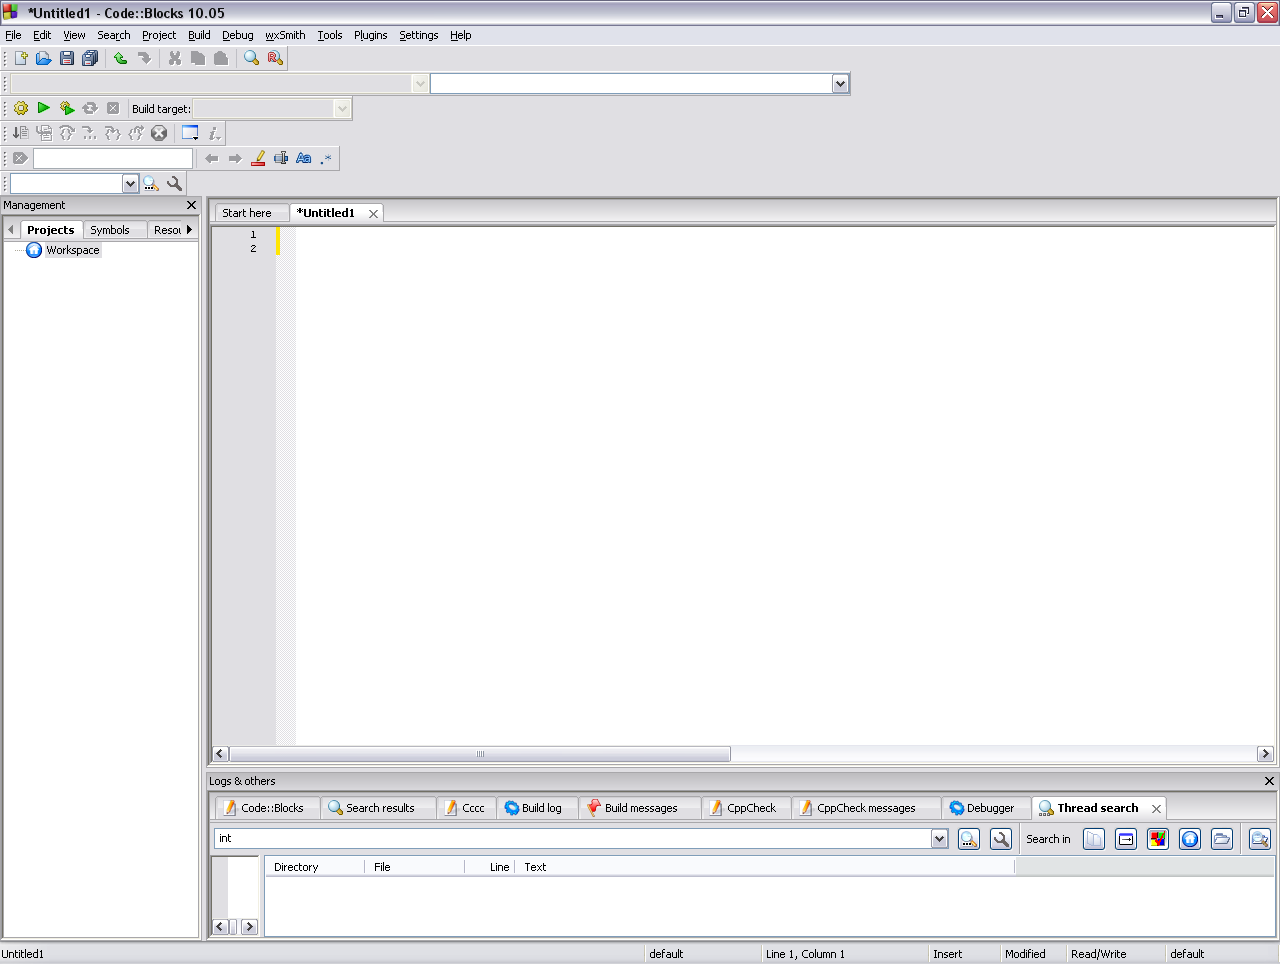
\includegraphics[scale=0.26]{images/cb_main}
\end{center}
\end{frame}

\begin{frame}{Елементи на главниот прозорец}
\begin{itemize}
  \item Лента со менија
    \begin{itemize}
      \item лентата со менија се наоѓа во најгорниот дел на прозорецот, веднаш под неговиот насловот 
      \item Во неа се наоѓаат менијата File, Edit, View, Search, Project, Build,
      Debug, wxSmith, Tools, Plugins, Settings, Help
    \end{itemize}
    \item Лента со алатки
    \begin{itemize}
      \item лентите со алатки (копчиња за стартување на најчесто користените
      команди на околината) се наоѓаат непосредно под лентата со паѓачки менија
    \end{itemize}
    \item Работна површина
    \begin{itemize}
      \item Потпрозорец за уредувачот на текст
      \item Прозорец за соопштенија.
      \item Прозорец за организација на работата на програмата
    \end{itemize}   
\end{itemize}
\end{frame}

\begin{frame}{Програмирање во C со Code::Blocks}{Креирање проект}
\begin{enumerate}
  \item Стартувајте CodeBlocks
  \item File -> New -> Project -> Empty Project -> Go 
\end{enumerate}
\begin{center}
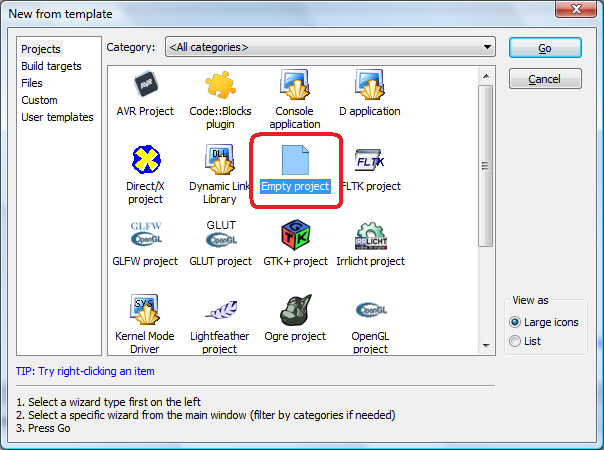
\includegraphics[scale=0.3]{images/cb_new}
\end{center}
\end{frame}

\begin{frame}{Програмирање во C со Code::Blocks}{Креирање проект}
\begin{enumerate}
\setcounter{enumi}{2}
  \item Одберете  GNU GCC Compiler
  \item Изберете ги следните 2 опции ако сакате да креирате “debug” и “release”
  configuration
\end{enumerate}
\begin{center}
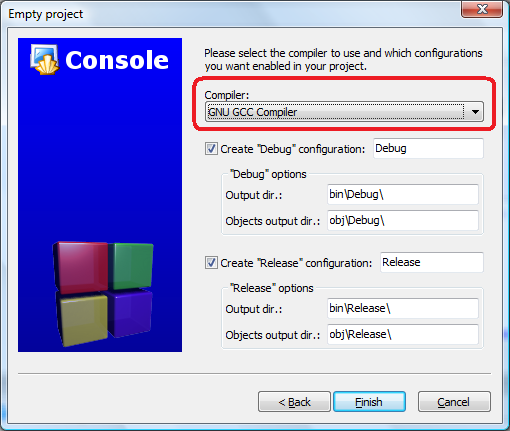
\includegraphics[scale=0.3]{images/cb_compiler}
\end{center}
\end{frame}

\begin{frame}{Додавање на изворна датотека}
\begin{enumerate}
\setcounter{enumi}{4}
  \item Додадете изворна датотека во проектот: File -> New -> File -> C/C++
  Source
  \item Одберете C како програмски јазик 
  \item Внесете го името на датотеката со полната патека и не заборавајте да го
  вклучите  "Add file to active project" 
\end{enumerate}
\begin{center}
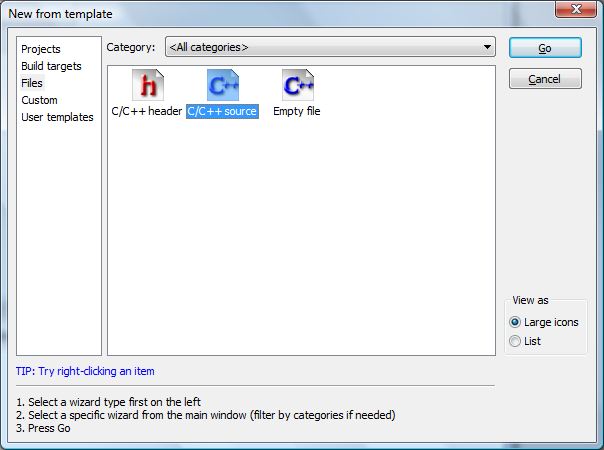
\includegraphics[scale=0.25]{images/cb_source}
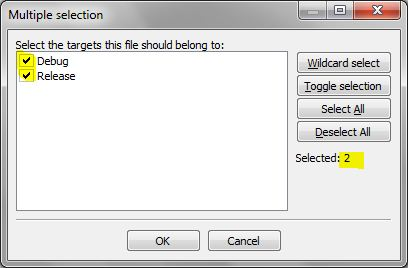
\includegraphics[scale=0.4]{images/cb_include}
\end{center}
\end{frame}

\begin{frame}{Програмирање}
\begin{itemize}
  \item За секој проект може да се постават следните опции "Project  Build Options..
Compiler Flags"
  \item За изградба на проектот (build) притиснете Ctrl + F9 
  \item За извршување на проектот притиснете Ctrl + F10
\end{itemize}
\begin{center}
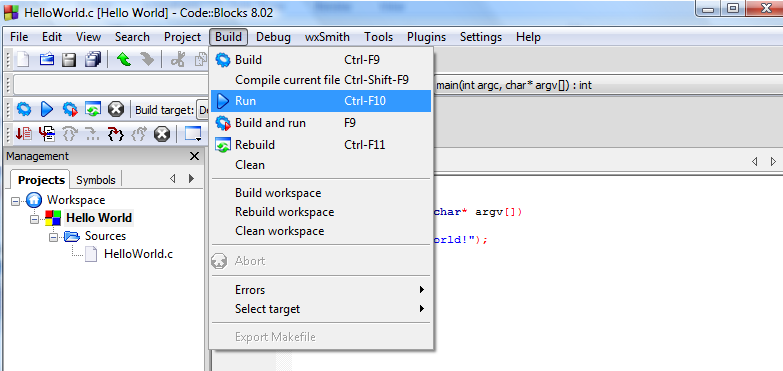
\includegraphics[scale=0.25]{images/cb_run}
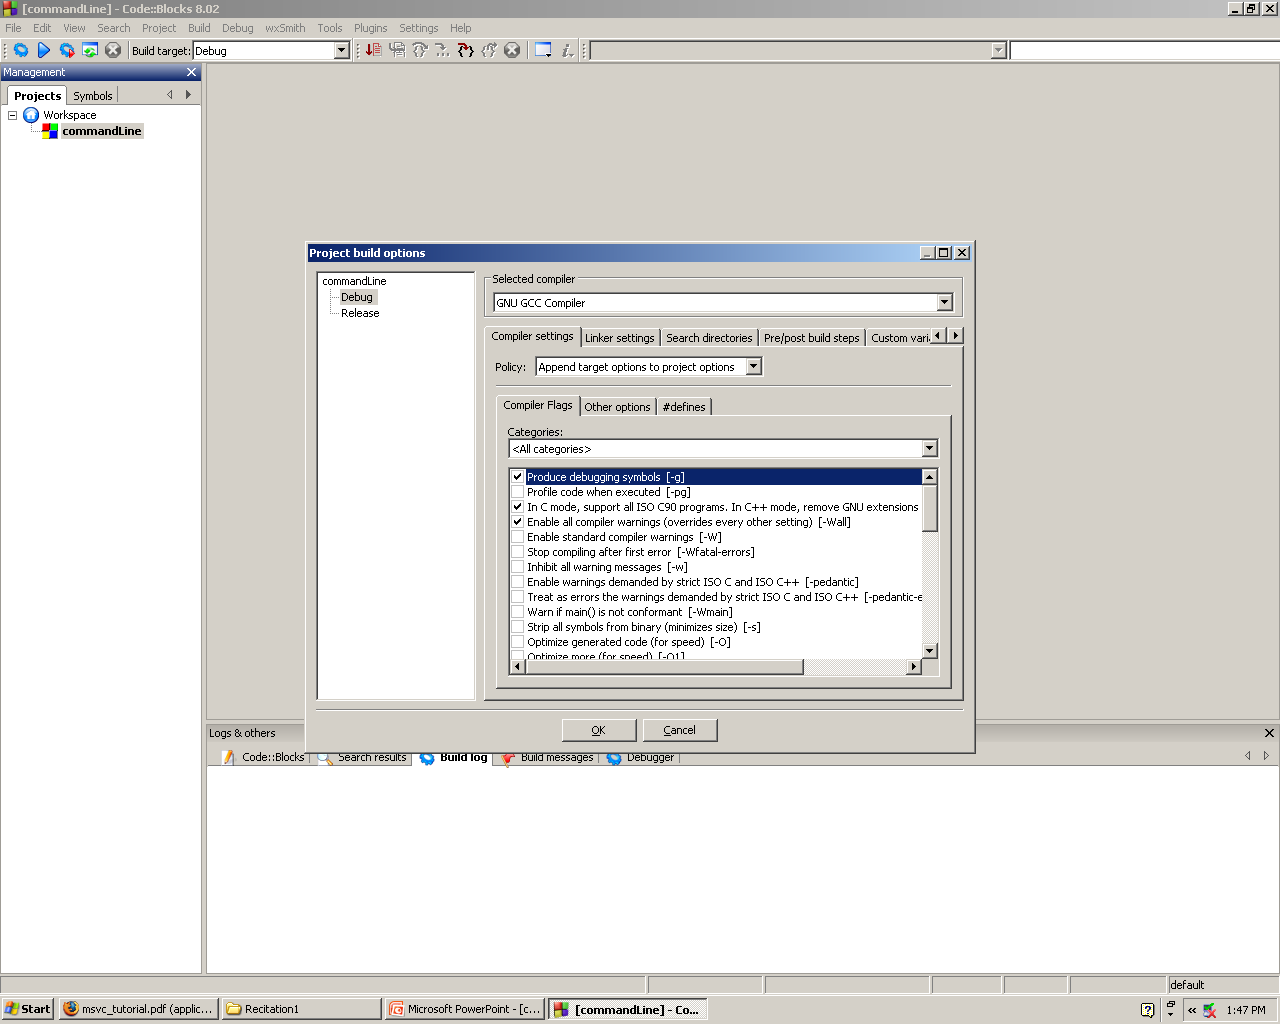
\includegraphics[scale=0.1]{images/cb_flags}
\end{center}
\end{frame}

\begin{frame}{Задачи за дома}
\begin{itemize}
  \item Во продолжение се наведени неколку задачи кои би требало да се обидете
  да ги изработите дома
  \item Со нивна изработка ќе бидете подготвени за успешна работа на
  претстојните лабораториски вежби
\end{itemize}
\end{frame}

\begin{frame}[fragile]{Задача 1}
Обидете се да креирате нов проект со една .с датотека и во неа внесете го
текстот на следнава програма:
\begin{lstlisting}
#include <stdio.h>

int main() {
    printf("Zdravo, kako si?\n");
    return 0;
}
\end{lstlisting}

\end{frame}

\begin{frame}{Задача 1}
\begin{itemize}
  \item Извршете ја програмата
\begin{itemize}
  \item Што добивате како резултат?
\end{itemize}
  \item Доколку сте направиле грешка при пишувањето на текстот поправете и
  извршете уште еднаш. 
  \item Направете намерно некоја грешка во текстот. Извршете повторно!
\begin{itemize}
  \item Што се случува сега?
\end{itemize}
\end{itemize}
\end{frame}

\begin{frame}[fragile]{Задача 2}
\definecolor{light-gray}{gray}{0.90}
Во текстот на програмата додадете до означениот ред:
\begin{lstlisting}[escapechar=!]
#include <stdio.h>
int main() {
    printf("Zdravo, kako si?\n");
    !\colorbox{light-gray}{printf("Neshto ne ti se pravi muabet?\n");}!
    return 0;
}
\end{lstlisting}
Кој е резултатот од извршувањето сега?
\end{frame}

\begin{frame}{Материјали и прашања}{}
    Предавања, аудиториски вежби, соопштенија\\
    \href{http://courses.finki.ukim.mk/}{\textbf{courses.finki.ukim.mk}}
    \vfill
    Изворен код на сите примери и задачи\\
    \href{http://bitbucket.org/tdelev/finki-krs/}{\textbf{bitbucket.org/tdelev/finki-krs}}
    \vfill
    Прашања и одговори\\
    \href{http://qa.finki.ukim.mk}{\textbf{qa.finki.ukim.mk}}
\end{frame}

\end{document}
